\documentclass[tikz, margin=2pt]{standalone}
\usepackage[utf8]{inputenc}
\usepackage[T1]{fontenc}

\usepackage{tikz}
\usepackage{helvet}
\usepackage{xcolor}
\usepackage{amsmath}

\renewcommand\familydefault\sfdefault
\newcommand{\DisplayDirectory}{0}

\usetikzlibrary{intersections, shapes.arrows, spath3, shapes.geometric, fit, backgrounds, calc}

\definecolor{themeBlue}{RGB}{1, 103, 143}
\definecolor{themeOrange}{RGB}{221, 109, 16}
\definecolor{themeTeal}{RGB}{18, 54, 69}
\definecolor{themeGrey}{RGB}{120, 121, 124}

\begin{document}
    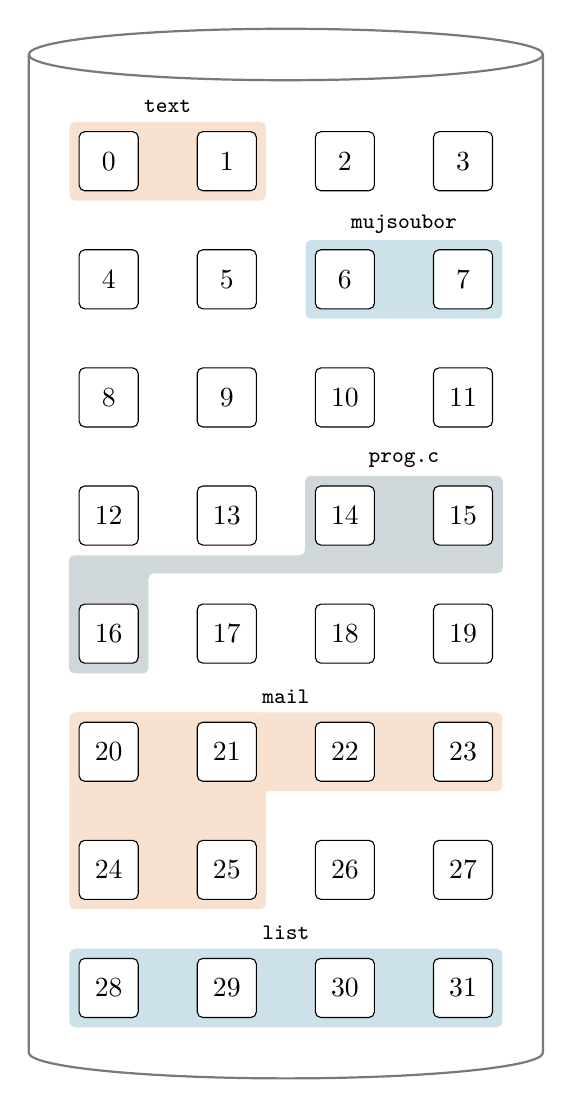
\begin{tikzpicture} [
        bus/.style={single arrow, single arrow head extend=2pt},
        l/.style={align=left},
        r/.style={align=right},
        c/.style={align=center}
    ]
        \foreach \y in {0, ..., 7} {
            \foreach \x in {0, ..., 3} {
                \pgfmathtruncatemacro{\label}{\x + (\y * 4)}
               \node [draw, minimum size=0.75cm, rounded corners=2pt, fill=white]  (\x\y) at (1.5*\x, -1.5*\y) {\label}; 
            }
        }
        
        \draw node[thick, cylinder, 
            draw = themeGrey, aspect=0.1, shape border rotate = 90, fit=(00) (37), inner sep=18pt] (c) {};
        
        \begin{scope}[on background layer]
            % FILE: text
            \draw node[fill=themeOrange!20, rounded corners=2pt, fit=(00) (10)] (0010) {};
            \draw (0010) ++(0, .7) node[font=\footnotesize] {\texttt{text}};
            
            % FILE: mujsoubor
            \draw node[fill=themeBlue!20, rounded corners=2pt, fit=(21) (31)] (2131) {};
            \draw (2131) ++(0, .7) node[font=\bfseries\footnotesize] {\texttt{mujsoubor}};
           
            % FILE: prog.c
            \fill[fill=themeTeal!20, rounded corners=2pt] 
                   ($ (23.north west) + (-3.5pt, 3.5pt) $) 
                to ($ (33.north east) + (3.5pt, 3.5pt) $) 
                to ($ (33.south east) + (3.5pt, -10pt) $) 
                to ($ (04.north east|-\tikztostart) + (3.5pt, 0) $) 
                to ($ (04.south east) + (3.5pt, -3.5pt) $) 
                to ($ (04.south west) - (3.5pt, 3.5pt) $) 
                to ($ (\tikztostart|-23.south west) - (0, 3.5pt) $)
                to ($ (23.south west|-\tikztostart) - (3.5pt, 0) $) 
                -- cycle;
            \draw ($ (23.north west)!.5!(33.north east) $) ++(0, .32) node[font=\footnotesize] {\texttt{prog.c}};
            
            % FILE: mail
            \draw node[fill=themeOrange!20, rounded corners=2pt, fit=(05) (35)] (0535) {};
            \draw node[fill=themeOrange!20, rounded corners=2pt, fit=(05) (16)] (0516) {};
            \draw (0535) ++(0, .7) node[font=\footnotesize] {\texttt{mail}};
        
            % FILE: list
            \draw node[fill=themeBlue!20, fit=(07) (37), rounded corners=2pt] (0737) {};
            \draw (0737) ++(0, .7) node[font=\footnotesize] {\texttt{list}};
        \end{scope}
    
        \ifnum\DisplayDirectory=1
            \matrix (table) [draw, text width=4em, font=\scriptsize, anchor=north] at ($ (c.north east|-c.after top) +(3, 0) $) {
                & \node[l] {\textbf{Soubor}};     & \node[r] {\textbf{Start}}; & \node[r] {\textbf{Počet}}; \\
                & \node[l] {\texttt{text}};       & \node[r] { 0 };            & \node[r] { 2 }; \\
                & \node[l] {\texttt{mujsoubor}};  & \node[r] { 6 };            & \node[r] { 2 }; \\
                & \node[l] {\texttt{prog.c}};     & \node[r] { 14 };           & \node[r] { 3 }; \\
                & \node[l] {\texttt{mail}};       & \node[r] { 20 };           & \node[r] { 6 }; \\
                & \node[l] {\texttt{list}};       & \node[r] { 28 };           & \node[r] { 4 }; \\
            };
            \draw (table.north) node[above, anchor=south, font=\footnotesize] {\textbf{Adresář}};
        \fi
    
    
    \end{tikzpicture}
\end{document}